\documentclass[10pt]{beamer}

%packages
\usepackage[english]{babel}
\usepackage[utf8]{inputenc}
\usepackage{graphicx}

%themes
\usetheme{Dresden}
\usecolortheme{rose}
\useoutertheme{tree}
\setbeamertemplate{caption}[numbered]

%general
\title{Poor harvest in India in 2002 shown with wheather Data Science}
\author{Tilman Hinnerichs, Anja Reusch}
\institute{Bertelsmann Data Science Scholarship Program}
\date{\today}

\begin{document}
\begin{frame}
	\titlepage
\end{frame}

\begin{frame}{What question would we like to answer?}
	On the search for good data we stumbled accross the CDC (Climate Data Center) of the DWD (German Wheather Center). They are providing data from all kinds of different wheather stations all around the world as we visualized in Figure~\ref{Stations}.
	\begin{figure}[ht]
		\centering
		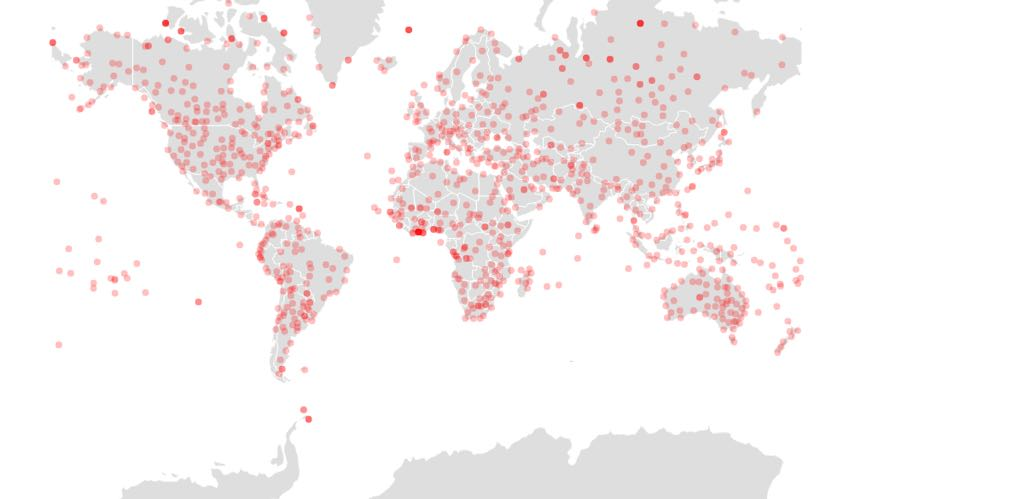
\includegraphics[width = 0.5\textwidth]{WheatherStations.jpeg}
		\caption{Wheather stations provided by the CDC}
		\label{Stations}
	\end{figure}
\end{frame}	

\begin{frame}{What question would we like to answer?}
	The CDC is providing all different kinds of data for those stations. Their database holds the statistics on snowfall, precipitation and sunshine hours and literally everything. The data is provided in a raw heap of data which we tried to classify.\\\vfill
	\large But what to do with that giant pile of data?
\end{frame}

\begin{frame}
	Hence, we found another source of data: The \textbf{Food and Agriculture Oranization of the United Nation}, which provides data on quantitative measurements of the yield of harvest. There we found a peak in the yield of paddled Rice of India in 2002, seen in Figure~\ref{IndiaRice}, where more than 22\% of the production got lost.
	\begin{figure}
		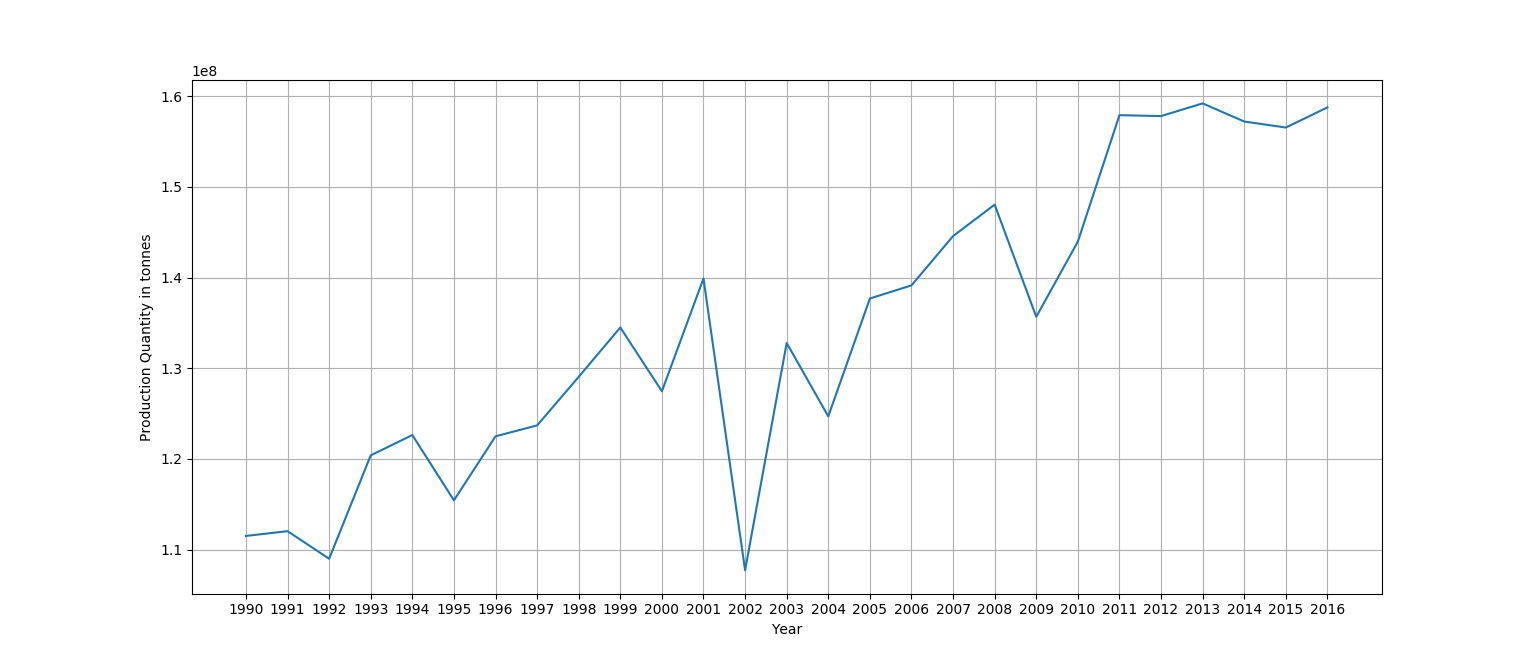
\includegraphics[width=1\textwidth]{IndiaRiceQuantity.png}
		\caption{We can see a harsh peek at 2002}
		\label{IndiaRice}
	\end{figure}
\end{frame}

\begin{frame}{What question would we like to answer?}
	So we would like to know: \\
	\begin{itemize}
		\item \large Can we see possible reasons for this peak in our wheather data?
	\end{itemize}
	
\end{frame}

\end{document}